% !TeX root = ../tcc.tex
\chapter{Revisão sistemática da literatura}
\label{cap:revisao-literatura}
\label{sec:conducao-revisao}

A revisão de literatura foi planejada para identificar e analisar evidências
sobre a avaliação de modelos de visão computacional aplicados a manifestações
cutâneas associadas à hanseníase. A definição de uma questão, de um protocolo,
de critérios de seleção e de procedimentos de extração e síntese é coerente
com as orientações de \citeonline{kitchenham2007} para revisões sistemáticas
em engenharia de software. O capítulo 4 de \citeonline[p. 51--56]{wohlin2024} apresenta a revisão
sistemática como estudo secundário e organiza seu processo em planejamento,
condução e relato. A obra fundamenta a definição de questões e critérios,
a documentação da busca, a seleção e a extração orientada pelas questões
de pesquisa. O procedimento
adotado nesta revisão é descrito a seguir; suas etapas não devem ser
interpretadas como a execução de um experimento controlado.

\section{Planejamento e protocolo}

O objetivo, o protocolo e os critérios foram organizados no Evidentia. A
questão principal é: como avaliar o desempenho de modelos de visão
computacional aplicados à identificação de padrões associados à hanseníase
em imagens de pele, no contexto da rede pública de saúde do Brasil? A
investigação foi detalhada nas seguintes questões secundárias:

\begin{enumerate}
\item Quais técnicas de visão computacional são usadas para identificar manifestações dermatológicas associadas à hanseníase?
\item Quais conjuntos de dados e populações são utilizados no desenvolvimento e na avaliação dos modelos?
\item Quais métodos e procedimentos são usados para avaliar o desempenho e quais resultados são relatados?
\item Quais métricas são usadas na avaliação e quais resultados são relatados?
\item Como o desempenho varia entre diferentes grupos ou tons de pele?
\item Quais modelos e abordagens de inteligência artificial são utilizados para identificar as manifestações dermatológicas associadas à doença?
\item Como a capacidade de generalização é avaliada, especialmente em conjuntos diferentes dos usados no treinamento?
\item Em que tipo de veículo o artigo foi publicado, como periódico ou conferência?
\end{enumerate}

\section{Estruturação da estratégia de busca}

Para estruturar a solicitação de busca, foram utilizados os componentes
registrados como população, contexto, intervenção e resultado do PICOC.
A população foi representada por termos de visão computacional,
inteligência artificial, redes neurais e aprendizado de máquina e profundo;
o contexto, por hanseníase e classificação ou segmentação de lesões
cutâneas; a intervenção, por modelos e arquiteturas de aprendizado de
máquina; e o resultado, por termos de avaliação, métricas e tarefas de
identificação. O \textit{prompt} preservado não apresenta um campo
separado de comparação. As perguntas e a relação completa de termos,
incluindo sinônimos e asteriscos, são reproduzidas no
Apêndice~\ref{ap:prompt-consensus}.

A Figura~\ref{fig:pico-pai} apresenta a representação PICO de
\citeonline{pai2004}, originalmente voltada à formulação de questões
clínicas. Nela, \textit{patient}, \textit{intervention}, \textit{comparison}
e \textit{outcome} correspondem, respectivamente, a paciente ou população,
intervenção, comparação e resultado. O PICOC acrescenta o contexto a esses
componentes. No procedimento deste trabalho, o \textit{prompt} utilizou
população, intervenção, contexto e resultado, sem campo específico de
comparação; a figura apresenta o modelo conceitual PICO e não afirma que
uma busca booleana exatamente igual à ilustrada foi executada.

\begin{figure}[htbp]
\centering
\caption{Representação dos componentes PICO para uma estratégia de busca}
\label{fig:pico-pai}
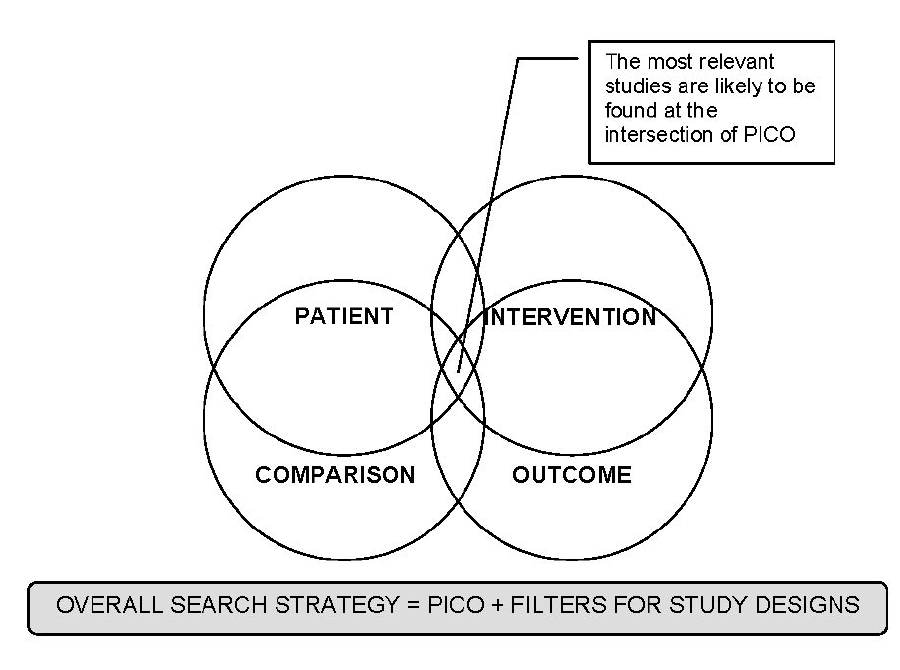
\includegraphics[width=0.68\textwidth]{figuras/pico-pai-2004.png}
\fonte{Reproduzido de \citeonline[p. 89, Figura 3]{pai2004}.}
\end{figure}

\subsection{Consultas apresentadas pelo Consensus}

Na busca de 25 de setembro de 2026, o Consensus apresentou uma sequência
de consultas em quatro rodadas. A Tabela~\ref{tab:consultas-consensus}
reproduz os textos e indicadores exibidos. Esses indicadores são saídas
internas da ferramenta, sem definição operacional disponível; não
correspondem a contagens auditadas de estudos únicos triados pela dupla.

\begin{longtable}{p{0.08\textwidth}p{0.68\textwidth}r}
\caption{Consultas e indicadores apresentados pelo Consensus}\label{tab:consultas-consensus}\\
\toprule
Rodada & Consulta & Indicador \\
\midrule
\endfirsthead
\toprule Rodada & Consulta & Indicador \\
\midrule
\endhead
1 & deep learning convolutional neural network leprosy Hansen disease skin lesion classification detection diagnosis & 95,3 mil \\
1 & U-Net ResNet EfficientNet Vision Transformer skin lesion segmentation leprosy hanseniasis dermatological pattern recognition & 2,3 mil \\
1 & machine learning model performance evaluation accuracy AUC F1 sensitivity specificity leprosy skin image diagnosis & 63,5 mil \\
1 & skin tone fairness demographic subgroup performance dermatology AI model external validation generalization cross-dataset & 67,4 mil \\
2 & leprosy skin image dataset Brazil public health AI diagnosis computer vision & 26,2 mil \\
2 & transfer learning self-supervised semi-supervised learning skin neglected tropical disease leprosy image classification & 36,6 mil \\
2 & WHO skin neglected tropical diseases mobile application telemedicine leprosy detection low-resource settings & 63,4 mil \\
3 & explainability XAI Grad-CAM interpretable AI leprosy neglected tropical disease skin lesion diagnosis & 1,6 mil \\
3 & histopathological image analysis acid-fast bacilli detection deep learning leprosy nerve biopsy microscopy & 17,6 mil \\
4 & leprosy skin image dataset multimodal clinical metadata paucibacillary multibacillary classification AI model & 3 mil \\
4 & reporting standards quality assessment QUADAS CONSORT-AI CLEAR dermatology AI model evaluation systematic review & 47,8 mil \\
\bottomrule
\end{longtable}

O painel informou ainda os indicadores \textit{Retrieved} de 425,4 mil,
\textit{Eligible} de mil e \textit{Included} de 100. Após a segunda
rodada, a ferramenta apresentou uma expansão por grafo de citações com dez
sementes e o indicador 662; após a terceira, indicou leitura de 12
resumos; antes da síntese, indicou leitura de resumos e PDFs de 100 itens.
O significado operacional desses indicadores, a identificação completa
das sementes e o acesso integral a cada PDF não foram comprovados. A
busca também foi ampliada para temas relacionados, como dermatologia geral,
equidade, saúde móvel, microscopia, histopatologia e diretrizes de relato;
nessas condições, a presença de uma referência na saída da ferramenta não
significa que ela atende aos critérios da revisão.


\section{Realização da busca e seleção dos artigos}
\subsection{Busca e identificação dos registros}

O protocolo da revisão foi organizado no Evidentia a partir da questão de
pesquisa e dos componentes do PICOC. Esses elementos foram utilizados em
uma solicitação em inglês ao Consensus, sem a inclusão dos critérios de
seleção no texto do \textit{prompt}. Em 25 de setembro de 2026, a
ferramenta retornou uma lista de 100 referências, das quais 98 tinham DOI
informado. Foi registrada também uma busca complementar por meio do Claude, da qual
foram reunidas 30 referências. A data, o \textit{prompt}, o modelo, a configuração e a lista completa
dessa busca complementar ainda precisam ser confirmados. Embora o protocolo
também registre a Scopus como fonte, não há comprovação de uma busca separada
nessa base na etapa descrita.

As duas listas somaram 130 registros e,
após a remoção de duplicatas, permaneceram 118 para triagem. A diferença
entre esses totais corresponde a 12 registros removidos; entretanto, os
pares considerados duplicados e o procedimento usado para identificá-los
ainda não foram integralmente documentados. O conjunto bibliográfico disponível contém 129 entradas. Na comparação
com os 118 registros triados, onze entradas não aparecem no conjunto de triagem e apresentam o mesmo DOI de outras entradas nele
representadas. Essa comparação permite identificar 11 pares de
registros com DOI coincidente, mas não identifica um eventual décimo
segundo registro removido nem comprova, isoladamente, quando cada par
foi deduplicado. A diferença entre as 129 entradas identificadas e os
130 registros informados no relato permanece a esclarecer. Os
indicadores internos apresentados pelo Consensus não foram tratados
como quantidades auditadas de estudos únicos examinados pelos pesquisadores.

\subsection{Critérios de seleção}

Os critérios de inclusão foram: disponibilidade do texto completo (CI01);
uso de visão computacional, aprendizado de máquina ou aprendizado profundo
para detectar, classificar, identificar ou segmentar manifestações
cutâneas humanas associadas à hanseníase (CI02); relato ou síntese de
evidências de avaliação de métodos de inteligência artificial para
hanseníase, incluindo experimentos, testes, validação ou comparação de
desempenho (CI03); uso, análise ou revisão de fotografias clínicas ou
imagens dermatoscópicas de lesões cutâneas humanas associadas à hanseníase
(CI04); e inclusão da hanseníase entre as condições avaliadas em trabalhos
que abordam múltiplas doenças (CI05). A formulação preservada do CI03 foi
recebida truncada após ``resultados de estu''; o trecho descrito acima
resume apenas a parte legível e sua redação integral deve ser confirmada.
Os critérios abrangem estudos primários e revisões, que devem ser
distinguidos durante a extração.

Foram informados os seguintes critérios de exclusão: registro duplicado de
artigo já considerado (CE01); publicação anterior a 2020 (CE02); texto
completo em idioma diferente de inglês ou português (CE03); uso exclusivo
de inteligência artificial generativa como intervenção (CE04); e ausência
de abordagem da hanseníase (CE05). A verificação de disponibilidade e
idioma do texto completo pode depender de consulta além do título e do
resumo, enquanto data e duplicidade também dependem dos metadados.

\subsection{Triagem e seleção para leitura integral}

O Jev Reviewer foi utilizado como apoio à classificação preliminar dos
118 registros. Para cada registro, suas sugestões são acompanhadas de
valores associados ao não atendimento de cinco critérios:
\begin{enumerate}
\item Abordar a hanseníase como condição investigada ou avaliada,
isoladamente ou entre outras doenças; uma menção apenas introdutória não
atende a esse critério.
\item Utilizar fotografias clínicas ou imagens dermatoscópicas de
manifestações cutâneas humanas associadas à hanseníase, ou revisar estudos
que utilizam essas imagens.
\item Aplicar ou analisar métodos de visão computacional, aprendizado de
máquina ou aprendizado profundo para detectar, classificar, identificar
ou segmentar essas manifestações nas imagens, incluindo revisões dessas
aplicações.
\item Relatar ou sintetizar evidências de avaliação desses métodos, como
experimentos, testes, validação, comparação de desempenho ou resultados
de estudos.
\item Não se limitar exclusivamente à inteligência artificial generativa
como intervenção.
\end{enumerate}

Esses cinco critérios descrevem o que foi avaliado pelo Jev; eles não
substituem os critérios gerais de inclusão e exclusão da revisão. Os valores
de \texttt{fails} acompanham a avaliação automatizada e não registram, por
si sós, a justificativa da decisão dos pesquisadores. Após a classificação
preliminar, a dupla relatou ter revisado os registros por título e resumo,
com as decisões registradas no Evidentia. A documentação não esclarece se
ambos avaliaram todos os registros de maneira independente. A avaliação por
dois ou mais pesquisadores, ao menos para uma amostra, é recomendada por
\citeonline[p. 55]{wohlin2024}; essa recomendação não demonstra que ela
foi executada neste trabalho.

As sugestões do Jev para os 118 registros foram: duas de inclusão, 15 incertas e 101 de exclusão.
O cruzamento por título entre as sugestões e as decisões do Evidentia
identificou correspondência para todos os registros. Entre os 26 com
situação de inclusão no Evidentia, dois tinham sugestão de inclusão do
Jev, 11 tinham sugestão incerta e 13 tinham sugestão de exclusão. Entre
os 91 excluídos no Evidentia, 87 tinham sugestão de exclusão e quatro
tinham sugestão incerta. O registro restante, classificado como
intermediário no Evidentia, tinha sugestão de exclusão pelo Jev. Assim,
as sugestões automáticas são distintas das decisões de triagem. A data de
execução, o modelo, a configuração completa e a versão da ferramenta não
foram identificados; os cinco critérios exibidos acima, por sua vez, estão
registrados nas avaliações disponíveis. Houve também discussão de exemplos de títulos e resumos com
o ChatGPT para apoiar a aplicação dos critérios; não é possível determinar
quantas decisões foram influenciadas por esse apoio.

Os estados intermediários da triagem registram, em uma etapa, 12 inclusões,
32 exclusões, 15 decisões intermediárias e 59 registros sem decisão. Em
outro estado foram observadas 19 inclusões, 40 exclusões e os mesmos 59
registros sem decisão; as 15 decisões intermediárias passaram a sete
inclusões e oito exclusões. As datas das decisões preenchidas indicam
28 de setembro de 2026, mas não registram horário de cada decisão. Esses
estados intermediários não devem ser confundidos com o resultado
consolidado descrito a seguir.

No Evidentia, 91 registros apresentam decisão de exclusão,
26 de inclusão e uma decisão intermediária, totalizando 118 registros.
Esse último registro, \textit{Leprosy Screening Based on Artificial
Intelligence: Development of a Cross-Platform App} \cite{souza2021}, apresenta duas
decisões individuais de exclusão, mas sua decisão consolidada foi
registrada manualmente como intermediária. Em outro registro,
\textit{Leprosy lesion recognition using convolutional neural networks} \cite{baweja2016},
houve uma decisão individual de inclusão e uma de exclusão; o conflito
foi resolvido manualmente com decisão consolidada de exclusão. Os demais
116 registros possuem decisão consolidada automática, segundo o campo
correspondente no Evidentia. Essa classificação descreve o mecanismo de
consolidação registrado pelo sistema e não identifica uma revisão
independente por ambos os pesquisadores para cada artigo.

A decomposição 91 exclusões, 26 inclusões e uma decisão intermediária
esclarece a diferença observada no registro anterior: 118 menos 26 é 92,
mas esse resultado reúne os 91 excluídos e o registro intermediário.
Assim, não se deve representar a diferença de 92 como 92 exclusões.
Os 26 registros com situação de inclusão na triagem constituem o conjunto
encaminhado à leitura integral, conforme o registro consolidado; esse
estado não comprova a elegibilidade definitiva após a leitura completa.

A Figura~\ref{fig:fluxo-triagem} sintetiza as quantidades descritas nesta
seção. A indicação de 12 registros removidos corresponde à diferença entre
130 e 118, ainda sujeita à reconciliação das fontes de identificação. O
resultado da leitura integral e o conjunto definitivo permanecem pendentes.

\begin{figure}[htbp]
\centering
\caption{Fluxo de identificação e triagem dos estudos}
\label{fig:fluxo-triagem}
\begin{tikzpicture}[
  box/.style={draw,rounded corners=2pt,align=center,text width=3.6cm,minimum height=1.0cm,inner sep=5pt,font=\small},
  wide/.style={box,text width=7.6cm},
  arrow/.style={-{Stealth[length=2.3mm]},thick}
]
\node[wide] (identified) {Registros informados: 130\\(Consensus: 100; Claude: 30)};
\node[wide,below=1.5cm of identified] (screened) {Registros após deduplicação: 118\\para triagem por título e resumo};
\draw[arrow] (identified) -- node[right=3mm,align=left,font=\scriptsize,text width=4cm] {12 registros: diferença\\calculada; a conciliar} (screened);
\node[box,below=1.15cm of screened,xshift=-4.3cm] (excluded) {Excluídos\\91 registros};
\node[box,below=1.15cm of screened] (included) {Incluídos na triagem\\26 registros};
\node[box,below=1.15cm of screened,xshift=4.3cm] (maybe) {Decisão\\intermediária\\1 registro};
\draw[arrow] (screened.south) -- ++(0,-0.45) -| (excluded.north);
\draw[arrow] (screened.south) -- (included.north);
\draw[arrow] (screened.south) -- ++(0,-0.45) -| (maybe.north);
\node[box,below=0.85cm of included] (fulltext) {Leitura integral\\e inclusão final\\pendentes};
\draw[arrow] (included) -- (fulltext);
\end{tikzpicture}
\fonte{Elaboração própria a partir dos resultados registrados no Evidentia e do histórico da busca.}
\end{figure}

\begin{table}[htb]
\centering
\caption{Quantidades documentadas na identificação e na triagem dos estudos}
\label{tab:fluxo-selecao-estudos}
\begin{tabular}{p{0.66\textwidth} r}
\toprule
Etapa ou registro & Quantidade \\
\midrule
Referências informadas do Consensus & 100 \\
Referências informadas do Claude & 30 \\
Registros reunidos, segundo o registro consolidado & 130 \\
Diferença entre os registros reunidos e os 118 para triagem & 12 \\
Entradas no conjunto bibliográfico disponível & 129 \\
Entradas ausentes da triagem com DOI coincidente & 11 \\
Registros na triagem do Evidentia & 118 \\
Excluídos na triagem & 91 \\
Incluídos na triagem & 26 \\
Decisão intermediária na triagem & 1 \\
Títulos presentes no formulário de extração & 25 \\
\bottomrule
\end{tabular}
\fonte{Elaboração própria a partir do registro da busca e das decisões de triagem.}
\end{table}

O formulário de extração contém 25 títulos que correspondem a
registros incluídos na triagem, enquanto os campos de extração estão
vazios. Entre os 26 incluídos no Evidentia, o registro
\textit{AI-generated dermatologic images show deficient skin tone
diversity and poor diagnostic accuracy: An experimental study} \cite{joerg2025} não
consta do formulário de extração. É necessário verificar a razão dessa
diferença, aplicar os critérios ao texto completo e registrar o resultado
antes de estabelecer o conjunto definitivo de estudos incluídos.

Os comentários do consenso e as notas disponíveis não registram o motivo
individual dos 91 registros excluídos; essa informação ainda deve ser
recuperada para permitir a verificação de cada decisão. As pontuações \texttt{fails} do Jev são associadas
a critérios, mas não constituem, por si sós, justificativas registradas
pelos revisores. Para completar a rastreabilidade do fluxo, ainda é
necessário recuperar os motivos de exclusão, esclarecer a diferença entre
as 129 entradas disponíveis e os 130 registros informados,
identificar o eventual décimo segundo registro removido e resolver a
situação intermediária. A quantidade incluída após a avaliação integral
ainda não foi confirmada.


\subsection{Extração e síntese das evidências}

Conforme \citeonline[p. 55--56]{wohlin2024}, o formulário de extração
deve ser orientado pelas questões de pesquisa e permitir o registro das
características dos estudos e dos dados necessários à síntese. Neste
trabalho, o formulário foi organizado para registrar título, autores,
ano, fonte, tipo de estudo e veículo, além das respostas às questões da
revisão: técnicas, bases de dados, populações, manifestações, quantidade de
imagens, métodos de avaliação, métricas, resultados, tons de pele,
modelos, generalização, validação e limitações. A leitura integral deverá
confirmar a elegibilidade e preencher esses campos com indicação da página,
seção ou tabela de origem. Estudos primários e revisões devem ser
identificados separadamente, para não atribuir aos revisores resultados de
experimentos relatados por outros autores.

A síntese deverá distinguir classificação, detecção e segmentação, bem
como resultados globais e específicos para hanseníase. Diferenças entre
grupos de tom de pele e evidências de generalização serão registradas
quando disponíveis; a ausência de resultados por grupo não será
interpretada como demonstração de equidade. A análise da aplicabilidade ao
contexto brasileiro não equivale a uma validação clínica. Até a conclusão
da leitura completa e da extração, a seleção e os resultados permanecem
provisórios.

\section{Resultados da revisão}
\label{sec:resultados-revisao}

Esta seção organiza a apresentação das evidências de acordo com as
questões secundárias da revisão. As observações a seguir retomam as
leituras já discutidas na introdução e identificam o que deverá ser
verificado na extração. Elas não representam uma síntese concluída dos
26 registros incluídos na triagem: a leitura integral e o preenchimento
do formulário ainda são necessários para confirmar o conjunto de estudos
e responder às questões de forma abrangente.

\subsection{Quais técnicas de visão computacional são utilizadas?}

As leituras iniciais ilustram o emprego de redes de aprendizado profundo
em tarefas distintas. \citeonline{yotsu2023} investigaram a classificação
de doenças com manifestações cutâneas; \citeonline{sanchez2024}, a
segmentação de feridas; e \citeonline{eita2025}, a localização e
classificação de lesões. A extração deverá identificar as técnicas e
distinguir as tarefas em cada estudo selecionado.

\subsection{Quais conjuntos de dados e populações são utilizados?}

A caracterização dos dados inclui a origem das imagens, a população, as
condições de aquisição e a quantidade de imagens disponíveis. Nos estudos
já examinados, \citeonline{yotsu2023} descrevem fotografias obtidas na
Costa do Marfim e em Gana, enquanto \citeonline{sanchez2024} apresentam
fotografias de feridas crônicas de pacientes com hanseníase. As demais
características e a comparação entre estudos dependem da extração.

\subsection{Quais métodos e procedimentos de avaliação são empregados?}

A análise deverá registrar os procedimentos de separação dos dados,
validação e comparação dos modelos, conforme forem apresentados em cada
artigo. Também será identificada a unidade de análise, como imagem,
paciente, objeto ou pixel. A descrição desses procedimentos ainda precisa
ser completada para o conjunto selecionado.

\subsection{Quais métricas e resultados são reportados?}

As medidas devem ser interpretadas de acordo com a tarefa executada. A
acurácia global em uma classificação multiclasse, por exemplo, não
representa necessariamente a sensibilidade para hanseníase. A análise das
matrizes de confusão apresentadas por \citeonline{yotsu2023} ilustra essa
distinção. As métricas consideradas na extração são apresentadas no
Capítulo~\ref{cap:referencial-teorico}; sua frequência e seus resultados
na revisão ainda serão apurados.

\subsection{Como o desempenho varia entre grupos ou tons de pele?}

A presença de imagens de diferentes tons de pele não demonstra, por si só,
equivalência de desempenho entre grupos. Em \citeonline{yotsu2023}, a
população das imagens é descrita, mas não são apresentados resultados
separados por fototipo. A revisão registrará comparações por grupo quando
houver informação suficiente; a ausência desses dados não permite concluir
que há equidade ou desigualdade de desempenho.

\subsection{Quais modelos e abordagens de inteligência artificial são empregados?}

Entre os trabalhos discutidos inicialmente estão MobileNetV2
\cite{jaikishore2021}, ResNet-50 e VGG-16 \cite{yotsu2023}, além de
YOLOv8 \cite{eita2025}. Esses exemplos demonstram a diversidade de
abordagens, mas não constituem uma contagem dos modelos encontrados no
conjunto final da revisão.

\subsection{Como a generalização dos modelos é avaliada?}

A análise de generalização deverá identificar se os autores avaliaram os
modelos em dados diferentes daqueles usados no treinamento e em quais
condições ocorreu essa avaliação. As evidências e limitações relativas à
generalização ainda precisam ser extraídas dos estudos selecionados.

\subsection{Em quais veículos os estudos são publicados?}

A classificação do veículo será registrada para cada estudo durante a
extração. Entre as leituras inicialmente utilizadas há publicações em
periódicos, como \citeonline{yotsu2023}, e em conferências, como
\citeonline{jaikishore2021}. A distribuição dos veículos no conjunto
final ainda não foi determinada.
